% generated by experiments/build_paper_assets.py -- do not edit by hand
\begin{figure}[t]
\centering
\resizebox{\linewidth}{!}{%
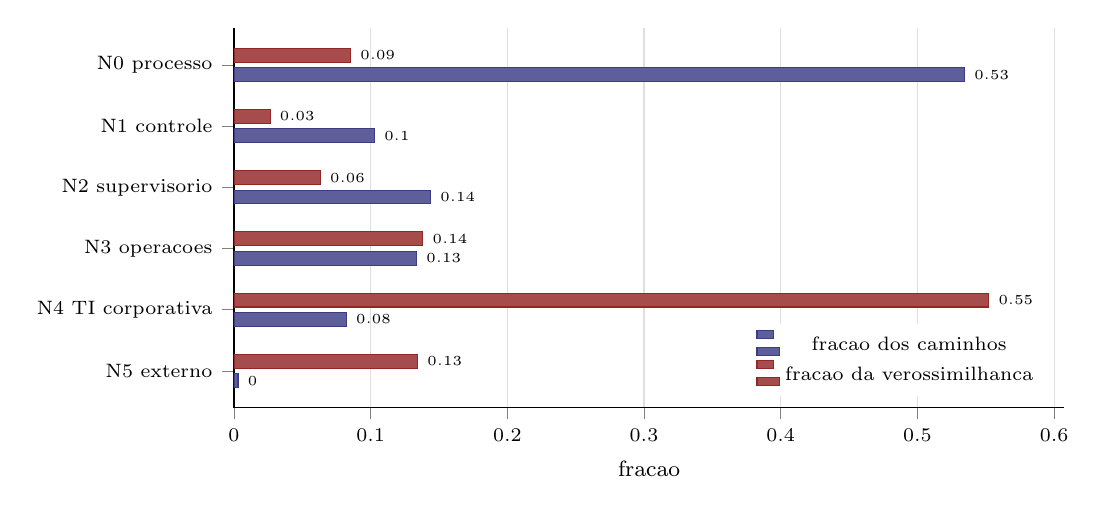
\begin{tikzpicture}
\begin{axis}[
    xbar, width=\linewidth, height=6.4cm,
    xlabel={fracao}, xmin=0,
    ytick={0,1,2,3,4,5}, yticklabels={{N0 processo},{N1 controle},{N2 supervisorio},{N3 operacoes},{N4 TI corporativa},{N5 externo}}, y dir=reverse,
    enlarge y limits=0.12, bar width=5pt,
    ticklabel style={font=\scriptsize}, label style={font=\footnotesize},
    nodes near coords, nodes near coords style={font=\tiny},
    every node near coord/.append style={/pgf/number format/fixed,
        /pgf/number format/precision=2},
    legend style={at={(0.98,0.03)}, anchor=south east, font=\scriptsize, draw=none},
    xmajorgrids, grid style={gray!25}, axis lines*=left, tick align=outside,
]
\addplot[fill=MidnightBlue!70, draw=MidnightBlue!85] coordinates {(0.534508,0) (0.102790,1) (0.143906,2) (0.133627,3) (0.082232,4) (0.002937,5)};
\addplot[fill=Maroon!70, draw=Maroon!85] coordinates {(0.085400,0) (0.026500,1) (0.063200,2) (0.138200,3) (0.552200,4) (0.134400,5)};
\legend{fracao dos caminhos, fracao da verossimilhanca}
\end{axis}
\end{tikzpicture}}
\caption{Onde o risco esta. Para cada nivel de Purdue, a fracao dos caminhos modelados que o alcancam como ponto mais profundo (barras a esquerda) contra a fracao da verossimilhanca agregada que esses caminhos carregam (barras a direita). A maioria dos caminhos desce fundo; a maior parte do risco plausivel nao.}
\label{fig:depth}
\end{figure}
